\section{Background}\label{sec:background}

% Prior study. Summary. Three major findings.
A prior study~\cite{con:hotpar12} browsed the bug databases of 46 real-world 
concurrency bugs and made three major findings on concurrency attacks. First, 
concurrency attacks are severe threats: 35 of the bugs can corrupt critical 
memory and cause three types of violations, including 
privilege escalations~\cite{uselib-bug-12791, mysql-bug-24988}, malicious code 
injections~\cite{berend-jan-wever-msiexploit}, and
bypassing security 
authentications~\cite{xwindows,theotheriphone,theotheriphone-2011}.

Second, concurrency bugs and attacks can often be easily triggered via subtle 
program inputs. For instance, attackers can use inputs to control the physical 
timings of disk IO and program loops and trigger concurrency bugs with a small 
number of re-executions. Third, compared to traditional TOCTOU attacks, which 
stem from corrupted file accesses, handling concurrency attacks is much more 
difficult because they stem from corrupted, miscellaneous memory accesses.

% Ineffectiveness of existing defense techniques.
These three findings reveal that concurrency attacks can largely weaken or 
even bypass most existing security defense tools, because these 
tools are mainly designed for sequential attacks. For instance, consider taint 
tracking tools, concurrency attacks can corrupt the metadata fields in these 
tools and completely bypass taint tracking. Anomaly detection tools, which rely 
on inferring adversary program behaviors (\eg, excessive re-executions), 
become ineffective, because concurrency attacks can easily manifest via subtle 
inputs.

% Introduce the question: what tool? Should be more directed here because the 
% prior study has shown the severity of concurrency attacks.
This prior study raises an open research question: \emph{what will be an 
effective tool for detecting concurrency attacks?} Specifically, can existing 
concurrency bugs detection tools effectively detect these bugs and their 
attacks? The answer is probably ``NO" because literature has overlooked these 
attacks.


\section{Quantitative Concurrency Attack Study}\label{sec:study}

% Study methodology. Studied XX real-world programs, including both applications 
% and kernels. Search CVE and open source bug databases with keywords. Manually 
% inspect the vulnerabilities. Use detection tools to detect these bugs if they 
% work with existing popular detection tools' platform (in total there are XX), 
% and inspected the number of total race reports, and inspect whether the race 
% reports have vulnerability implications.


% Our study, exclude tocttou, exclude repeated ones, added XX extra attacks, 
% finally identify 27 attacks.

We studied concurrency attacks in \nprog widely used programs, including 3 
servers, 2 browsers, 1 library, and 4 kernel distributions. We 
added the shared memory concurrency bugs in the prior 
study~\cite{con:hotpar12}, and we searched ``concurrency bug vulnerability" in 
CVE and these programs' bug databases. We manually inspected bug reports 
and removed them if they were false reports or lack a clear description, and 
we conservatively kept the vulnerable ones caused by multithreading.

Unlike the prior study~\cite{con:hotpar12} which counted the number of 
security consequences in bug reports as the number of concurrency attacks, 
we counted only each bug's first security consequence. In total we collected 
\nattacks concurrency attacks with three more types of violations than the 
prior study~\cite{con:hotpar12}, including HTML integrity violations 
(\S\ref{sec:unknown-attacks}), buffer overflows (\S\ref{sec:example}), and DoS 
attacks (\S\ref{sec:unknown-attacks}). We built scripts to successfully exploit 
\nreproduced attacks in \nreproducedProgs programs if we had source code.

To quantitatively analyze why concurrency attacks are overlooked, we  
considered data race detectors because they have effectively 
found concurrency bugs. We selected two popular tools: \tsan~\cite{tsan:wbia09} 
for applications and \ski~\cite{ski:osdi14} for OS kernels. We ran the two 
tools on \nreproducedProgs programs that support these tools. We used the 
programs' common performance benchmarks as workloads. 
Table~\ref{tab:study} shows a study summary.
% Our study also considerfed bug 
% consequence analysis tools and anomaly detection tools. 

% Prog order: from app to kernel; in app, from server to others; alphabetical.
\begin{table}[h]
\footnotesize
\centering
\vspace{-.1in}
\begin{tabular}{lrrrr}
{\bf Name} & {\bf LoC}  & {\bf \# Concurrency attacks}  & 
{\bf \# Race reports} \\
\hline\\[-2.3ex]
% apps
%\moonlight                &    TBD   &    1 &    N/A \\
%\kde                      &    TBD   &    2 &    N/A \\
% kernels
%\macos                    &    TBD   &    2 &    N/A \\
\apache                     &    290K  &    4 &    715  \\
\mysql                      &    1.5M  &    2 &    1123 \\
\ssdb                       &    67K   &    1 &    12  \\
\chrome                     &    3.4M  &    3 &    1715 \\
\iexplorer                  &    N/A   &    1 &    N/A \\
\libsafe                    &    3.4K  &    1 &    3   \\
% \libvirt                    &    680K  &    1 &    0 \\
\linux                      &    2.8M  &    8 &    24641 \\
\darwin                     &    N/A   &    3 &    N/A \\
\freebsd                    &    680K  &    2 &    N/A \\
\windows                    &    N/A   &    1 &    N/A \\
\hline\\[-2.3ex]
Total                       &    8.0M  & \nattacks & 28209 \\
\end{tabular}
\vspace{-.1in}
\caption{{\em Concurrency attacks study results.} \rm {This table contains both 
known and previously unknown concurrency attacks we detected. We 
made \nreproducedProgs out of \nprog programs run with race 
detectors. We built exploit scripts for \nreproduced concurrency 
attacks in these \nreproducedProgs programs.}} 
\label{tab:study}
\vspace{-.15in}
\end{table}



\subsection{Challenging Findings}\label{sec:findings}



%\begin{figure}[h]
%\centering
%\includegraphics[width=0.8\columnwidth]{figures/apache}
%%\vspace{-.1in}
%\caption{{A concurrency attack in the \apache web server.}} \label{fig:apache}
%\vspace{-.15in}
%\end{figure}



% These attacks allow attackers to 
% corrupt critical memory, overflow heaps and stacks, inject malicious code, 
% escalate programs' privileges, and bypass authentication checks. 

\para{I: Concurrency attacks are much more severe than concurrency bugs.} Every 
studied program has concurrency attacks. Figure~\ref{fig:libsafe} shows a 
concurrency attack that bypassed stack overflow checks in the 
\libsafe~\cite{libsafe} library and injected malicious 
code. Figure~\ref{fig:uselib} shows a concurrency attack in the Linux \uselib 
system call. Attackers have leveraged this bug to trigger a NULL pointer 
dereference in the kernel and execute arbitrary code from user space.

One key difference between concurrency attacks and concurrency 
bugs is that fixing the buggy code is not sufficient to fix the 
vulnerabilities. For instance, once attackers have got OS root 
privileges~\cite{freebsd-exploit-2009-3527,uselib-bug-12791}, they may stay 
forever in the system. Therefore, it's still crucial to study whether existing 
known concurrency bugs may lead to concurrency attacks.

\begin{figure}[h]
\vspace{-.1in}
\centering
\includegraphics[width=0.8\columnwidth]{figures/libsafe}
\vspace{-.55in}
\caption{{A concurrency attack in the \libsafe security library. } 
\rm{Dotted arrows mean the bug-triggering thread interleaving. When Thread 2 
detects a stack overflow attack, it sets the \v{dying} variable to 1 and kills 
current process shortly. However, access to \v{dying} is not correctly 
protected 
by mutex, so Thread 1 reads this variable, bypasses the security check in
\v{stack\_check()} (called at line 164), and runs into a 
stack overflow in \v{strcpy()} (at line 165).}}
\label{fig:libsafe}
\end{figure}

\begin{figure}[h]
\centering
% \vspace{-.03in}
\includegraphics[width=0.9\columnwidth]{figures/kernel_uselib_msync}
\vspace{-.25in}
\caption{{A concurrency attack in the Linux \uselib and \v{msync()} system 
calls. }\rm{Dotted arrows mean the bug-triggering thread interleaving. A data 
race on the \v{f\_op} struct causes the Linux kernel to trigger a NULL 
pointer dereference and enables arbitrary code execution.}} 
\label{fig:uselib}
\vspace{-.1in}
\end{figure}

%\para{Concurrency attacks are more than just TOCTOU attacks.}
%Concurrency attacks are much broader than the TOCTOU attacks
%studied by previous work due to two main reasons. First, the TOCTOU attacks in 
%previous work target primarily the file access interface (\eg, \v{open()} 
%and \v{access()}). This interface allows users to check file permissions and 
%use file data but does not directly support transactions that make the check and 
%the use atomic. An attacker may thus exploit this limitation to gain illegal 
%file accesses. In contrast, the concurrency attacks we studied target general 
%memory access interface (\eg, \v{load} and \v{store} instructions), corrupt a 
%program's global memory (\eg, via data races), and lead to various types of 
%vulnerabilities.

% Heming: don't mention many buggy patterns because our front ends only have 
% data race detectors for now.
% Second, the TOCTTOU races in previous work exhibit one specific interleaving 
% pattern: atomicity violations where the check and the use is not atomic. In 
% contrast, our study reveals various interleaving patterns, including data 
% races, atomicity violations, order violations [25] where a set of accesses
% is supposed to occur in a fixed order, but no synchronizations
% % enforce the order.

%Second, as a natural fallout of the first reason, techniques proposed by 
%previous TOCTOU work are too specific to detect or prevent general concurrency 
%attacks. For instance, while launching a TOCTOU attack requires concurrent 
%executions, the vulnerable program may be purely sequential, so TOCTOU 
%detectors may not need to reason about concurrency at all. Similarly,
%TOCTOU detectors may mediate all file system calls without high runtime 
%overhead, but it would be prohibitive to mediate all load or store 
%instructions to detect data races.

\para{II: Concurrency bugs and their attacks are widely spread in program 
code.} Among \nreproduced attacks we had source code and constructed exploit 
scripts, \nreproducedInter have their bugs and vulnerability sites among 
different functions. Moreover, bugs often affect vulnerability sites not only 
through data flows but also control flows (\eg, the \libsafe attack in 
Figure~\ref{fig:libsafe}).

This finding suggests that a concurrency attack detection tool should 
incorporate both inter-procedural and control-flow analyses. Unfortunately, to 
scale to large programs, existing bug consequence analysis tools 
(\eg,~\cite{conseq:asplos11,yamaguchi:sp14,livshits05finding}) lack 
either inter-procedural or control-flow analysis.

\para{III: Concurrency bugs and their attacks are often triggered by separate, 
subtle program inputs.} Consider the inputs to trigger 
concurrency bugs, unlike previous 
understanding~\cite{pres:sosp09,cui:tern:osdi10} that 
triggering concurrency bugs require intensive repeated executions, 
\nreproducedNoRetry out of the
\nreproduced reproduced concurrency attacks in our study can be easily 
triggered with less than 20 repetitive executions on our evaluation machines 
with carefully chosen program inputs. For instance, in a \mysql 
privilege escalation~\cite{mysql-bug-24988}, we used the ``\v{flush 
privileges;}" query to trigger a data race and corrupted another \mysql user's 
privilege table with only 18 repeated executions.

In addition to input values, carefully crafted input timings can also expand 
the \emph{vulnerable window}~\cite{con:hotpar12} which increases the chance of 
running into the bug-triggering schedules. For 
instance, consider Figure~\ref{fig:uselib}, since the \v{if} statement and the  
\v{file->f\_op->fsync()} statement in \v{msync\_interval()} have an IO 
operation (not shown) in between, attackers could craft inputs with subtle timings 
for this IO operation and thus enlarged the time window of these two statements. 
Then, attackers could easily trigger the buggy schedule in Figure~\ref{fig:uselib}.

In addition to the inputs for triggering concurrency bugs, triggering the 
attacks of these bugs often require other subtle program inputs. A main 
reason is the bugs and their attacks are widely spread in program 
code and thus they may easily be affected by different inputs. In a Linux 
\uselib data race~\cite{uselib-bug-12791}, 
we needed to carefully construct kernel swap IO operations to trigger the race, 
and we needed to call extra system calls to get a root shell out of this race. 
By constructing subtle inputs for both the bug and its attack, we needed only 
tens of repeated executions to get this root shell on our evaluation machines.

This \uselib attack reveals two issues. First, a small number of repeated 
executions indicates that attackers can easily bypass anomaly detection 
tools~\cite{schonberg:pldi89,taskrecycling:ppopp90,diduce:icse02} 
with subtle inputs. Second, existing data race detectors are ineffective at 
revealing this attack because they will stop after they run a bug-triggering input 
and flag this race report. Such a one-shot detection will overlook a 
concurrency attack as it often requires extra inputs to trigger the attack. 
Therefore, extra analysis is required to identify the bug-to-attack propagation.

% TBD: heming, emphasis not only functions, but also indirect control flow 
% propagation. E.g., libsafe.
% TODO: Concurrency attacks are not necessarily only located in certain part of 
% the program code.

\para{IV: Most concurrency bugs that triggered concurrency attacks can be 
detected by race detection tools.} There are several types of concurrency bugs,
including data race, atomicity violation, 
and order violation~\cite{lu:concurrency-bugs}. Although some types of 
concurrency bugs are difficult to detect (\eg, order violation), we found that 
all concurrency bugs we studied were data races and these bugs can readily be 
detected by \tsan or \ski. This finding suggests that a race detector 
is a necessary component for detecting concurrency attacks.
% The only exception is the atomicity 
% violation bug in \libvirt (see Table~\ref{tab:study}). 

% This finding suggests 
% that data race detection tools should be a necessary component in a concurrency 
% attack detection system.

% Since the root cause of concurrency 
% attacks is concurrency bugs, it is vital to identify the associated concurrency 
% bugs in order to identify concurrency attacks. 
% However, not all types of 
% concurrency bugs can be detected by well used exisiting tools,

\para{V: Concurrency attacks are overlooked mainly due to the excessive 
reports from race detectors.} We identified two major reasons for this finding. 
First, existing race detectors generate too many bug reports which deeply bury 
the vulnerable ones. For instance, we ran \mysql with \tsan and repeatedly 
generated the same bug-triggering SQL query~\cite{mysql-bug-24988}. We got 
\nmysqlDetectedSameReq race reports, but after our manual inspection, only two 
reports will lead to attacks. Table~\ref{tab:study} shows 
more programs with even more reports. These excessive reports make 
finding concurrency attacks from the reports just like ``finding needles in a 
haystack."

Second, even if a developer luckily opens a true bug report that can actually 
lead to an attack, she still has no clue whether what attacks the bug may lead 
to, because the report only shows the bug itself (\eg, the corrupted variable), 
but not its security consequences. Therefore, it's crucial to have an analysis 
tool that can accurately identify the bug-to-attack propagation for bug reports.

% Heming: hack, make the arch figure locate at the same page as section 4.2.
\begin{figure*}[!tbh]
\centering
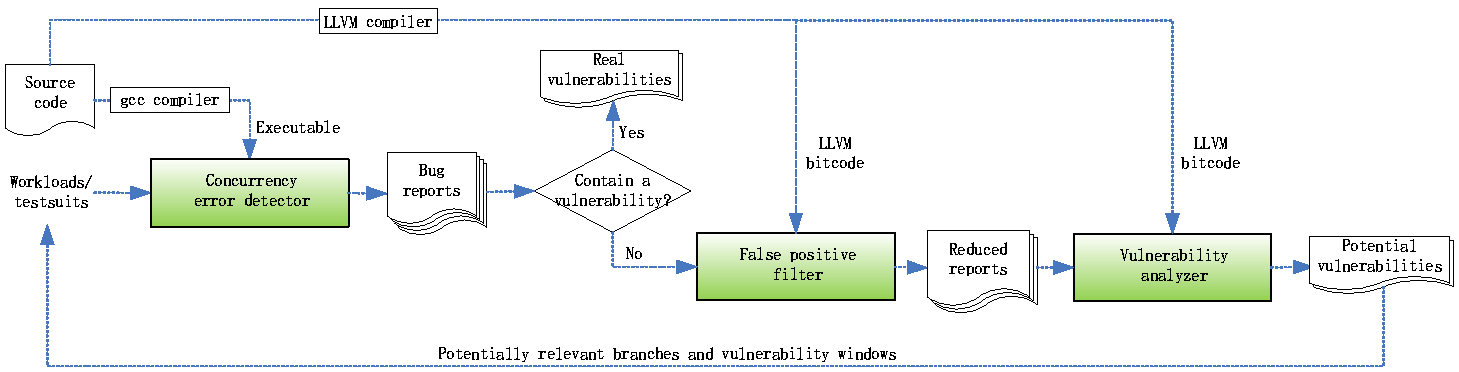
\includegraphics[width=0.7\textwidth]{figures/arch}
\vspace{-.20in}
\caption{{\em The \xxx Architecture.} \rm {\xxx components are the blue 
(shaded) ones.}} \label{fig:arch}
\vspace{-.2in}
\end{figure*}

\subsection{Optimistic Findings}\label{sec:patterns}

To assist the construction of a practical concurrency attack detection tool, 
we identified two common patterns for concurrency attacks. First, although the 
consequences of concurrency attacks are miscellaneous, these consequences are 
triggered by five explicit types of vulnerable sites, including memory 
operations (\eg, \v{strcpy()}), NULL pointer deferences, privilege operations 
(\eg, \v{setuid()}), file operations (\eg, \v{access()}), and process-forking 
operations (\eg, \v{eval()} in shell scripts). Our study found that these 
vulnerable sites have independent consequences to each other, thus more types 
can be easily added.


Second, concurrency bugs and their attacks often share similar call stack 
prefixes. From the \nreproduced concurrency attacks with source code, 
\nreproducedInter of them have the vulnerability site in the callees (\ie, the 
call stack of the bug is a prefix of the call stack of the vulnerability site). 
For the rest them, the vulnerability site is just one or two levels up of the 
bug's call stack. These two patterns reveal an opportunity to build a precise, 
scalable static analysis tool for tracking the bug-to-attack propagation.

% the corrupted memory of concurrency 
% attacks rarely propagate through return values of function calls. This is 
% probably due to the corrupted memory is global varible or heap, but not stack 
% variables. 

% First, because 
% concurrency attacks tend to leverage the corrupted memory that resides during a 
% program's execution, the propagation from the corrupted memory to a 
% vulnerability action widely 
% spreads across branch instructions and function calls. For instance, 5 
% concurrency attacks we studied incurred at least XX branch instructions or 
% function calls. This long propagation distance indicates that existing 
% consequence-oriented analysis tools (\eg,~\cite{conseq:asplos11}) for 
% concurrency bugs may work poorly on concurrency attacks.




